% \documentclass{report}

% \usepackage{hyperref}  % package for linking figures etc
% \usepackage{enumitem}  % package for description with bullets
% \usepackage{graphicx}  % package for importing images
% \usepackage{mathtools} % package for math equation
% \usepackage{mathrsfs}  % package for math font
% \usepackage{indentfirst} % package for getting ident after section or paragraph
% % \usepackage{amsmath}

% \setlength{\parindent}{2em} % how much indent to use when we start a paragraph

% \graphicspath{ {./theory/figures/} }       % path for images

% \begin{document}

\chapter{Background}


\section{Machine Learning}

\subsection{Introduction}
Machine Learning (ML) is a field which is raised out of Artificial Intelligence (AI). Applying AI, we wanted to build better and intelligent
machines. But except for few mere tasks such as finding the shortest path between point A and B, we were unable to program more complex
and constantly evolving challenges. There was a realisation that the only way to be able to achieve this task was to let machine learn
from itself. This sounds similar to a child learning from its self. So machine learning was developed as a new capability for computers.
And now machine learning is present in so many segments of technology, that we don’t even realise it while using it. \par
Finding patterns in data on planet earth is possible only for human brains. The data being very massive, the time taken to compute is
increased, and this is where Machine Learning comes into action, to help people with large data in minimum time. \\
There are three kinds of Machine Learning Algorithms :
 
\begin{enumerate}
\item Supervised Learning
\item Unsupervised Learning
\item Reinforcement Learning
\end{enumerate}

\subsubsection{Supervised Learning}
A majority of practical machine learning uses supervised learning. In supervised learning, the system tries to learn from the previous examples that are given. Speaking mathematically, supervised learning is where you have both input variables (\textit{x}) and output variables (\textit{Y}) and can use an algorithm to derive the mapping function from the input to the output. The mapping function is expressed as
$Y = f(x)$.
\begin{figure}[h]
  \centering
  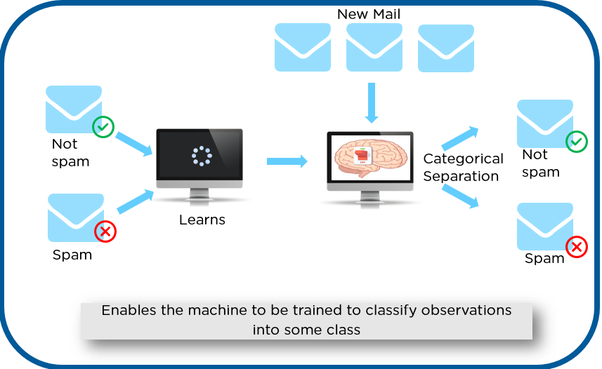
\includegraphics[scale=0.3]{supervised_leaning_example2}
  \caption{Example of supervised Learning}
  \label{fig:supervised_learning_example}
\end{figure}

As shown in Figure \ref{fig:supervised_learning_example}, we have initially taken some data and marked them as ‘Spam’ or ‘Not Spam’. This
labeled data is used by the training supervised model, in order to train the model. Once it is trained, we can test our model by testing it with some test new mails and checking of the model is able to predict the right output. 

Supervised learning problems can be further divided into two parts, namely \textbf{classification}, and \textbf{regression}.
\begin{description}
\item[ Classification] : A classification problem is when the output variable is a category or a group, such as “black” or “white” or “spam” and “no spam”.
\item[ Regression ] :  A regression problem is when the output variable is a real value, such as “Rupees” or “height.”
\end{description}
Some Supervised learning algorithms include:
\begin{itemize}
\item Decision trees
\item Support-vector machine
\item Naive Bayes classifier
\item k-nearest neighbors
\item linear regression
\end{itemize}

\subsubsection{Unsupervised Learning}

In unsupervised learning, the algorithms are left to themselves to discover interesting structures in the data. Mathematically, unsupervised
learning is when you only have input data (\textit{X}) and no corresponding output variables. This is called unsupervised learning because
unlike supervised learning above, there are no given correct answers and the machine itself finds the answers.
\begin{figure}[h]
  \centering
  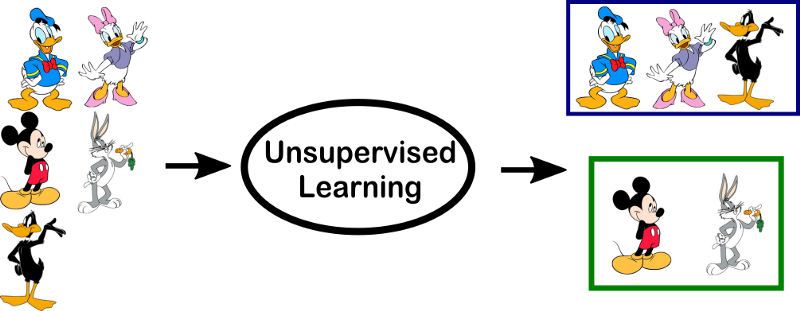
\includegraphics[scale=0.3]{unsupervised_learning_example}
  \caption{Example of unsupervised Learning}
  \label{fig:unsupervised_learning_example}
\end{figure}
In Figure \ref{fig:unsupervised_learning_example}, we have given some characters to our model which are ‘Ducks’ and ‘Not Ducks’. In our
training data, we don’t provide any label to the corresponding data. The unsupervised model is able to separate both the characters by
looking at the type of data and models the underlying structure or distribution in the data in order to learn more about it. Unsupervised
learning problems can be further divided into \textbf{association} and \textbf{clustering} problems.

\begin{description}
\item[ Association] : An association rule learning problem is where you want to discover rules that describe large portions of your data, such as “people that buy X also tend to buy Y”.
\item[ Clustering] : A clustering problem is where you want to discover the inherent groupings in the data, such as grouping customers by purchasing behaviour.
\end{description}

\subsubsection{Reinforcement Learning}
A computer program will interact with a dynamic environment in which it must perform a particular goal (such as playing a game with an
opponent or driving a car). The program is provided feedback in terms of rewards and punishments as it navigates its problem space. 
Using this algorithm, the machine is trained to make specific decisions. It works this way: the machine is exposed to an environment
where it continuously trains itself using trial and error method.
\begin{figure}[h]
  \centering
  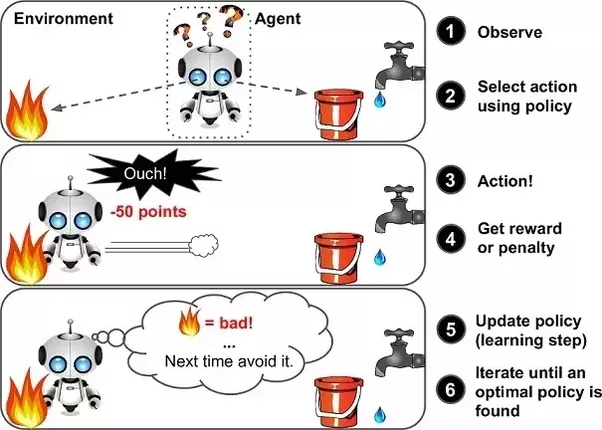
\includegraphics[scale=0.3]{reinforment_learning_example}
  \caption{Example of Reinforcement Learning}
  \label{fig:reinforment_learning_example}
\end{figure}
In Figure \ref{fig:reinforment_learning_example}, we can see that the agent is given 2 options i.e. a path with water or a path with fire. A reinforcement algorithm
works on reward a system i.e. if the agent uses the fire path then the rewards are subtracted and agent tries to learn that it should avoid
the fire path. If it had chosen the water path or the safe path then some points would have been added to the reward points, the agent then
would try to learn what path is safe and what path isn’t

\subsection{Neural Networks}
Neural Networks are a class of models within the general machine learning literature. Neural networks are a specific set of algorithms that
have revolutionized the field of machine learning. They are inspired by biological neural networks and the current so called deep neural
networks have proven to work quite very well. Neural Networks are themselves general function approximations, that is why they can be applied
to literally almost any machine learning problem where the problem is about learning a complex mapping from the input to the output space.

\subsection{A single Neuron}
The basic unit of computation in a neural network is the neuron, often called a \textbf{node} or \textbf{unit}. It receives input from some
other nodes, or from an external source and computes an output. In purely mathematical terms, a neuron in the machine learning world is a
placeholder for a mathematical function, and its only job is to provide an output by applying the function on the inputs provided.
Each input has an associated weight (\textit{w}), which is assigned on the basis of its relative importance to other inputs. The node applies
a function \textit{f  (defined below)} to the weighted sum of its inputs as shown in Figure \ref{fig:Perceptron}.
\begin{figure}[h]
  \centering
  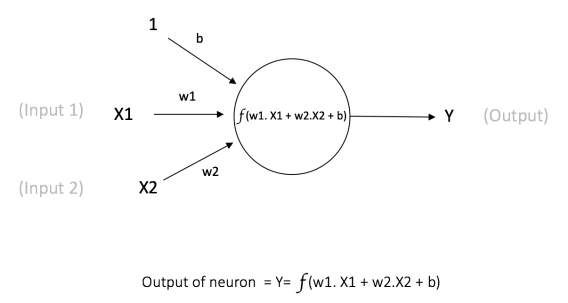
\includegraphics[scale=1.0]{perceptron}
  \caption{An example of a single Neuron}
  \label{fig:Perceptron}
\end{figure}
The network takes numerical inputs \textit{X1} and \textit{X2} and has weights \textit{w1} and \textit{w2} associated with those inputs.
Additionally, there is another \textit{input 1} with weight \textit{b} (called \textit{Bias}) associated with it. The main function of Bias is to provide every node with a trainable constant value (in addition to the normal inputs that the node receives). The output Y from the neuron
is computed as shown in the Figure \ref{fig:Perceptron}. The function \textit{f} is non-linear and is called \textbf{Activation Function}. The
purpose of the activation function is to introduce non-linearity into the output of a neuron. This is important because most real world data
are non linear and we want neurons to learn these non-linear representations.
\subsubsection{Activation Functions} 
Every activation function (or non-linearity) takes a single number and performs a certain fixed mathematical operation on it. There are
several activation functions:
\begin{description}
\item[ Sigmoid ] : takes a real-valued input and squashes it to range between 0 and 1. Its formula is:
  \[ \sigma(x) = \frac{1}{1 + e^{-x} } \]
  It is easy to understand and apply but it has major reasons which have made it fall out of popularity:
  \begin{itemize}
  \item Vanishing gradient problem
  \item Its output isn’t zero centered. It makes the gradient updates go too far in different directions.
  \item Sigmoids saturate and kill gradients.
  \item Sigmoids have slow convergence.
  \end{itemize}

\item [ Tanh ] : takes a real-valued input and squashes it to the range [-1, 1]. Its formula is:
  \[ tanh(x) = 2 \sigma(2x) -1 \]
  Now it’s output is zero centered because its range in between -1 to 1. Hence optimization is easier in this method and  in practice it is always preferred over Sigmoid function . But still it suffers from Vanishing gradient problem.

\item[ ReLU ]: ReLU stands for \textit{Rectified Linear Unit}. It takes a real-valued input and thresholds it at zero (replaces negative values with zero). So its formula is:
  \[ f(x) = max(0,x) \]
  It has become very popular in the past couple of years. It was recently proved that it had 6 times improvement in convergence from Tanh
  function. Seeing the mathamatical form of this function we can see that it is very simple and efficinent . A lot of times in Machine
  learning and computer science we notice that most simple and consistent techniques and methods are only preferred and are best.
  Hence it avoids and rectifies vanishing gradient problem . Almost all deep learning Models use ReLu nowadays.
\end{description}

Figure \ref{fig:Activation}  show each of the above activation functions.
\begin{figure}[h]
  \centering
  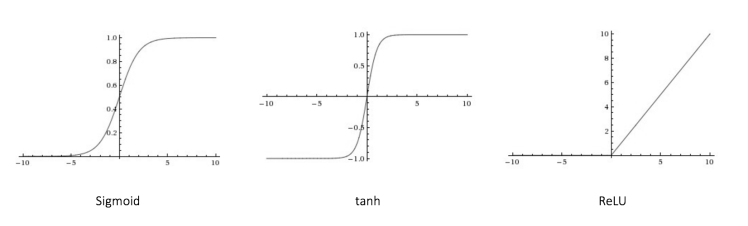
\includegraphics[scale=1.0]{activation_figures}
  \caption{Plots of Activation functions}
  \label{fig:Activation}
\end{figure}

\subsubsection{Feedforward Neural Network}
Till now we have covered neuron and activation functions which together for the basic building blocks of any neural network. The feedforward
neural network was the first and simplest type of artificial neural network devised. It contains multiple neurons (nodes) arranged in layers.
A layer is nothing but a collection of neurons which take in an input and provide an output. Inputs to each of these neurons are processed
through the activation functions assigned to the neurons. Nodes from adjacent layers have connections or edges between them. All these connections have weights associated with them.
\begin{figure}[h]
  \centering
  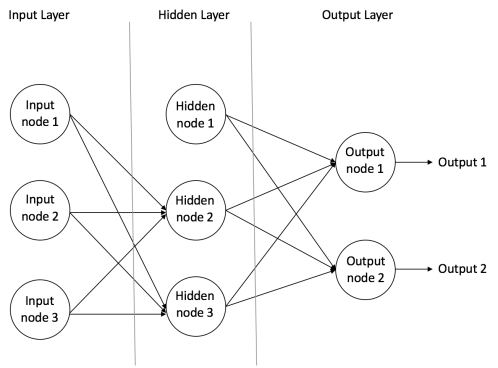
\includegraphics[scale=1.0]{feedforwardnetwork}
  \caption{An example of a Feedforward Neural Network}
  \label{fig:feedforwardnetwork}
\end{figure}
An example of a feedforward neural network is shown in Figure \ref{fig:feedforwardnetwork}. A feedforward neural network can consist of three types of nodes:
\begin{description}
\item[ Input Nodes ] The Input nodes provide information from the outside world to the network and are together referred to as the
  “Input Layer”. No computation is performed in any of the Input nodes – they just pass on the information to the hidden nodes.
\item[  Hidden Nodes ]  The Hidden nodes have no direct connection with the outside world (hence the name “hidden”). They perform
  computations and transfer information from the input nodes to the output nodes. A collection of hidden nodes forms a “Hidden Layer”.
  While a feedforward network will only have a single input layer and a single output layer, it can have zero or multiple Hidden Layers.
\item [ Output Nodes ] The Output nodes are collectively referred to as the “Output Layer” and are responsible for computations and
  transferring information from the network to the outside world.
\end{description}

In a feedforward network, the information moves in only one direction – forward – from the input nodes, through the hidden nodes (if any)
and to the output nodes. There are no cycles or loops in the network (this property of feed forward networks is different from Recurrent
Neural Networks in which the connections between the nodes form a cycle). Another important point to note here is that each of the hidden
layers can have a different activation function, for instance, hidden layer1 may use a sigmoid function and hidden layer2 may use a ReLU,
followed by a Tanh in hidden layer3 all in the same neural network. Choice of the activation function to be used again depends on the
problem in question and the type of data being used.

\subsection {2D Convolutional Neural Network}
A Convolutional Neural Network (ConvNet/CNN) is one of the variants of neural networks used heavily in the field of Computer Vision. It
derives its name from the type of hidden layers it consists of. The hidden layers of a CNN typically consist of convolutional layers, pooling
layers, fully connected layers, and normalization layers. Here it simply means that instead of using the normal activation functions defined
above, convolution and pooling functions are used as activation functions.
It can take in an input image, assing importance (learning weights and biases) to various aspects/objects in the image and be able to
differentiate one from the other. The pre-processing required in a ConvNet is much lower as compared to the other classification algorithms.
While in primitive method filters are hand-engineered, with enough training, ConvNets have the ability to learn these filters/characteristics.

The architecture of a ConvNet is analogous to that of the connectivity pattern of Neurons in the Human Brain and was inspired by the
structure of the Visual Cortex. However, most ConvNets costist mainly in 2 parts:
\begin{description}[font=$\bullet$\scshape\bfseries]
\item [ Feature extractor] : \\
  This part of the network takes as input the image and extract features that are meaningful for its classification. It amplifies aspects
  of the input that are important for discrimination and suppresses irrelevant variations. Usually, the feature extractor cosists of
  several layers. For instance, an image which could be seen as an array of pixel values. The first layer often learns reprensations
  that represent the presence or absence of edges at particular orientations and locations in the image. The second layer typically
  detects motifs by spotting particular arrangements of edges, regardeless of small variations in the edge positions. Finally, the third
  may assemble motifs into larger combinations that correspond to paths of familiar objects, and subsequent layers would detect objects
  as combinations of these parts.
  
\item [ Classifier ] : \\
  This part of the network takes as input the previously computed features and use them to predict the correct label.
\end{description}

\begin{figure}[h]
  % 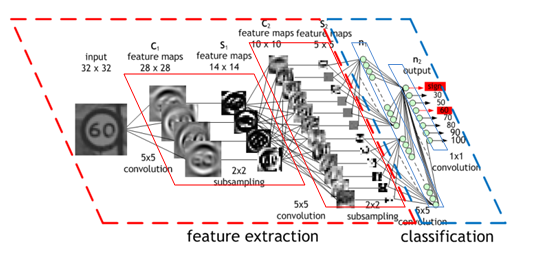
\includegraphics[scale=0.7]{convolutional_neural_network_structure} \]
  \centering
  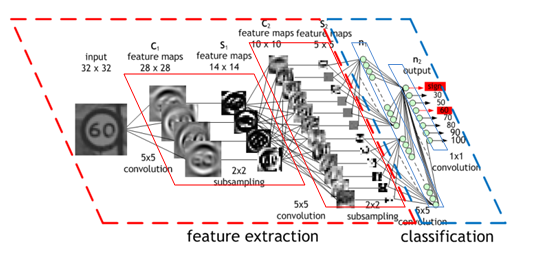
\includegraphics[scale=0.7]{convolutional_neural_network_structure}
  \caption{Typical structure of a ConvNet}
\end{figure}
\paragraph{Convolutional Layers}
In order to extract such features, ConvNets use 2D convolution operations. These operations take place in convolutional layers. Convolutional
layers consist of a set of learnable filters. Every filter is small spatially (along widht and height), but extends through the full depth of
input. During forword pass, we slide (more precisely, convolve) each filter across the width and height of the input volume and compute dot
products between the entries of the filter and the input at any position (as Figure \ref{fig:conv_example} shows). The objective of the
Convolution Operation is to extract the high-level features such as edges, from the input image. ConvNets need not be limited to only one
Convolutional Layer. Conventionally, the first ConvLayer is responsible for capturing the Low-Level features such as edges, color, gradient
orientation, etc. With added layers, the architecture adapts to the High-Level features as well, giving us a network which has the wholesome
understanding of images in the dataset, similar to how we would.

\begin{figure}[h]
  \centering
  \begin{minipage}[b]{0.4\textwidth}
    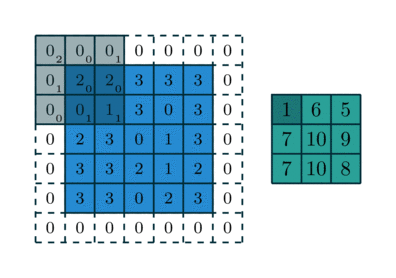
\includegraphics[width=\textwidth]{conv_1}
  \end{minipage}
  \hfill
  \begin{minipage}[b]{0.4\textwidth}
    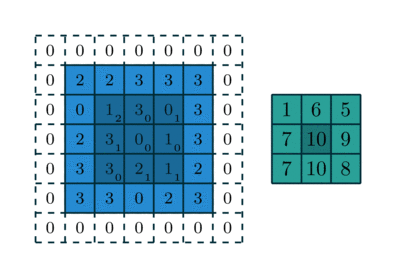
\includegraphics[width=\textwidth]{conv_2}
  \end{minipage}
  \caption{Convolution with kernel size:3, stride:2, padding:1}
  \label{fig:conv_example}
\end{figure}
\paragraph{Pooling Layers}
\subsection{3D Convolutional Neural Network}
Traditionally, ConvNets are targeting RGB images (3 channels). The goal of 3D CNN is to take as input a video and extract features from it.
When ConvNets extract the graphical characteristics of a single image and put them in a vector (a low-level representation), 3D ConvNets
extract the graphical characteristics of a set of images. 3D CNNs takes in to account a temporal dimension (the order of the images in the
video). From a set of images, 3D CNNs find a low-level representation of a set of images, and this representation is useful to find the
right label of the video (a given action is performed). \\
In order to extract such features, 3D ConvNets  use 3D convolution operations.
\begin{figure}[h]
  % 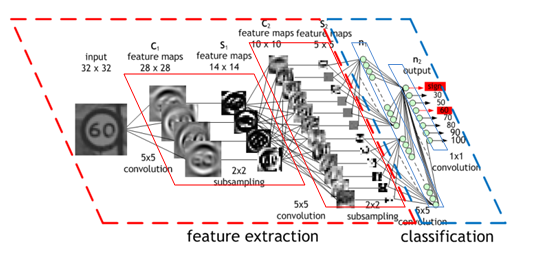
\includegraphics[scale=0.7]{convolutional_neural_network_structure} \]
  \centering
  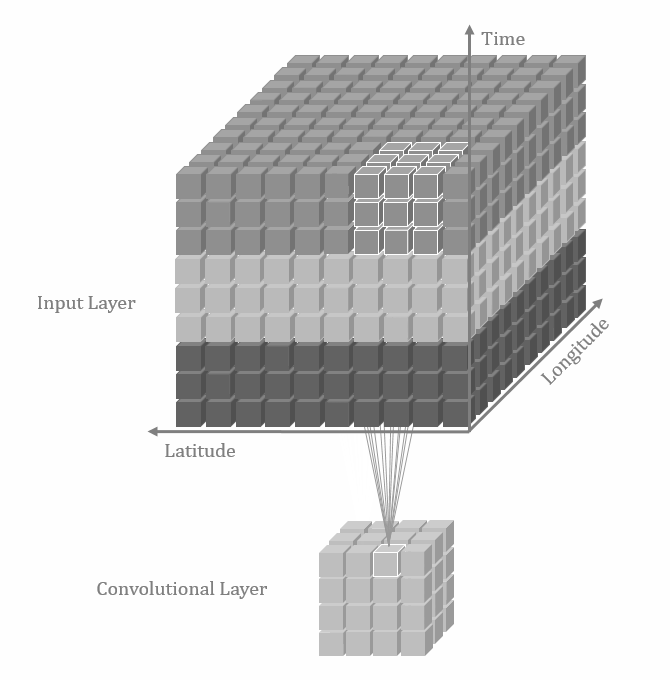
\includegraphics[scale=0.3]{3d_conv}
  \caption{3D Convolution operation}
\end{figure}

There are several existing approaches to tackle the video classification. This is a nonexaustive list of existing approaches:
\begin{description} [font=$\bullet$\scshape\bfseries]
\item[ ConvNets + LSTM cell] : Extract features from each frame with a ConvNet, passing the sequence to an RNN
\item[ Temporal Relation Networks] : Extract features from each frame with a ConvNet and pass the sequence to an MLP
\item[ Two-Stream Convolutional Networks] : Use 2 CNN, 1 spatial stream ConvNet which process one single frame at a time, and 1 Temporal stream ConvNet which process multi-frame optical flow
\end{description}

\section{Object Detection}
Within the field of Deep Learning, the sub-discipline called “Object Detection” involves processes such as identifying the objects through a picture, video or a webcam feed.
Object Detection is used almost everywhere these days. The use cases are endless such as Tracking objects, Video surveillance, Pedestrian detection etc. 
An object detection model is trained to detect the presence and location of multiple classes of objects. For example, a model might be trained with images that
contain various pieces of fruit, along with a label that specifies the class of fruit they represent (e.g. an apple, a banana, or a strawberry),
and data specifying where each object appears in the image.

The main process followed by most of CNN for Object Detection is:
\begin{enumerate}
\item Fistly, we do feature extraction using as backbone network, the first Convolutional Layers of a known pre-trained CNN such
  as AlexNet, VGG, ResNet etc.
\item Then, we propose regions of interest (ROI) in the image. These regions contain possibly an object, which we are looking for.
\item Finally, we classify each proposed ROI.
\end{enumerate}

\subsection{ Region Proposal Network}

From the 3 above steps, the 2nd step is considered to be very important. That is because, in this step, we should choose regions of
the image, which will be classified. Poor choice of ROIs means that the CNN will pass by some object that are located in the image,
because, they were not be proposed to be classified.

\begin{figure}[h]
  \centering
  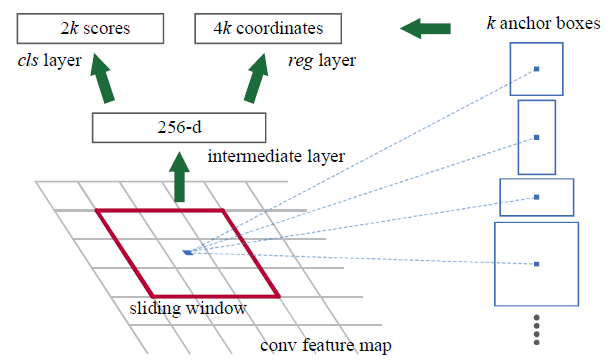
\includegraphics[scale=0.3]{RPN_structure}
  \caption{ Region Proposal Network's structure}
  \label{fig:rpn_structure}
\end{figure}

The first Object-Detection CNNs use several algorithms for proposing ROIs. For example, R-CNN\cite{DBLP:journals/corr/GirshickDDM13},
and Fast R-CNN\cite{Girshick:2015:FR:2919332.2920125} used Selective Search Algorithm for extracting ROIs.
One of noverlties introduced by the Faster R-CNN\cite{Ren:2015:FRT:2969239.2969250} is \textbf{Region Proposal Network} (RPN). Its
Function is to propose ROIs and its structure can be shown in \ref{fig:rpn_structure}. As we can see, RPN is consisted of:
\begin{itemize}
\item 1 2D Convolutional Layer
\item 1 score layer 
\item 1 regression layer
\end{itemize}

Another basic element of RPN is the \textbf{anchors}. Anchors are predefined boxes used for extracting ROIs. In figure \ref{fig:anchors} is
depicted an exaple of some anchors
\begin{figure}[h]
  \centering
  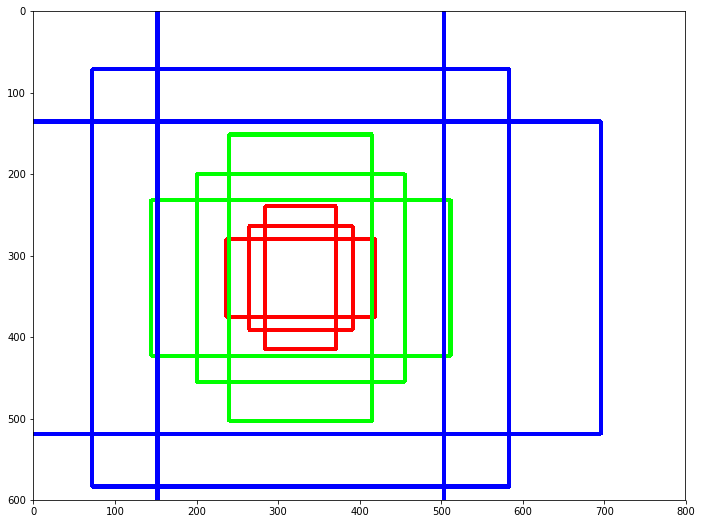
\includegraphics[scale=0.3]{anchors}
  \caption{ Anchors for pixel (320,320) of an image (600,800) }
  \label{fig:anchors}
\end{figure}

For each feature map's pixel corresponds \textbf{k (k=9)} anchors (3 different scales and 3 different ratios 1:1, 1:2, 2:1). \par
As a result, RPN gets as input feature maps extracted from the backbone CNN. Then performs 2D convolution over this input and passes
the output to its scoring layer and regression layer. Those scores represent the confidence of existing an object in this specific position.
On top of that, regression layer outputs 4k displacements, 4 for each anchor. Finally, we keep as output only the \textit{ n-best scoring} anchors.

\section{Losses and Metrics}
In order to train our model and check its performance, we use some known Loss functions and Metrics used in Object Detection systems.
\subsection{Losses}
For training our network, we use \textbf{Cross Entropy Loss} for classification layers and \textbf{smooth L1-loss} for regression.
\subsubsection{Cross Entropy Loss}
TODO
\subsubsection{Smooth L1-loss}
TODO
\subsection{Metrics}
Evaluating our machine learning algorithm is an essential part of any project. The way we choose our metrics influences how the performance
of machine learning algorithms is measured and compared.
They influence how to weight the importance of different characteristics in the results and finally, the ultimate choice of which algorithm to choose. Most of the times we use classification accuracy
to measure the performance of our model, however it is not enough to truly judge our model.

\subsection{Precision, Recall \& F1 score}

\begin{description}
\item[ Precision ]  measures how accurate is your predictions. i.e. the percentage of your predictions are correct.
\item[ Recall ] measures how good you find all the positives. For example, we can find 80\% of the possible positive cases in our top K predictions.
\end{description}
Their definisions are:
\[ Precision = \frac{TP}{TP + FP} \]  
\[  Recall = \frac{TP}{TP + FN} \] 
\[ F1 = 2 \cdot \frac{precision \cdot recall}{precision + recall} \]
where \begin{itemize}
\item TP = True positive
\item TN = True negative
\item FP = False positive
\item FN = False negative
\end{itemize}

\subsection{Intersection over Union}

Intersection over Union (IoU)  measures the overlap between 2 boundaries. We use that to measure how much our predicted boundary overlaps with the ground truth (the real object boundary).
In some datasets, we predefine an IoU threshold (say 0.5) in classifying whether the prediction is a true positive or a false positive.



\subsection{mAP}
Precision and recall are single-value metrics based on the whole list of predictions. By looking their formulas, we can see that there is
a trade-off between precision and recall performance. This trade-off can be adjusted by the softmax threshold, used in model's final layer.
In order to have high precision performance, we need to decrease the number of FP. But this will lead to decrease recall performance and
vice-versa. \par
As a result, these metrics fail to determine if a model is performing well in object detection tasks as well as action detection tasks. For
that reason, we use mAP metric
\paragraph{AP (Average precision)} is a popular metric in measuring the accuracy of object detectors like Faster R-CNN, SSD, etc. Average precision computes the average precision value for recall value over 0 to 1.

In our case, we use the metrics presented in \cite{DBLP:journals/corr/GkioxariM14} in
order to quantify our results:
\begin{description}
\item[ frame-AP ] measures the area under the precision-recallcurve of the detections for each frame (similar to the PASCAL  VOC  detection  challenge  \cite{Everingham10}).   A  detection is correct
  if the intersection-over-union with theground truth at that frame is greater than and the ac-tion label is correctly predicted.
\item [ video-AP ] measures the area under the precision-recallcurve of the action tubes predictions. A tube is correctif the mean per frame intersection-over-union with theground truth across the
  frames of the video is greaterthan and the action label is correctly predicted.
\item [ AUC ] measures the area under the ROC curve, a metricpreviously used on this task.  An action tube is correctunder the same conditions as invideo-AP. Following
  \cite{Tian:2013:SDP:2514950.2515975} , the ROC curve is plotted until a false positive rateof 0.6, while keeping the top-3 detections per class andper video. Consequently,
  the best possible AUC scoreis 60\%.
\end{description}



% \end{document}